\def\Titel{Die Gedanken sind frei}  
\def\WorteUndWeise{Wort \& Weise: Deutsches Volkslied}
\def\Referenz{Horst: 123} %Falls auf die Seitenzahl eines anderen Liederbuchs verwiesen werden soll. Bsp.: \def\Referenz{Horst: 123}

%Titel für das Inhaltsverzeichnis. Alle Titel-Varianten mit je einem /index Befehl auflisten.
\index{Die Gedanken sind frei}
\index{Gedanken}

%Nur eine Variante auswählen! Die andere mit % auskommentieren oder löschen.
\LiedSetup{}               %Nur Inhaltsverzeichnis
%\EinSchnellesLiedSetup{}   %Inhaltsverzeichnis + Ein schnelles Lied!

\begin{guitarMagic}

    [e]Akkorde werden in eckige Klammer an die Stelle geschrieben \\
    [H7]über welcher sie stehen sollen.\\
    Man kann einen Akkord auch über einen Bereich zentrieren, \\
    indem man diesen in [e]{geschweiften} Klammern direkt dahinter schreibt.
    
    Wenn ein Akkord in eine Lücke geschrieben werden soll, \\
    muss davor und dahinter ein [E] Leerzeichen sein. \\
    Einen Zeilenumbruch erzeugt man mit doppelten Backslachs \\
    und einen neuen Absatz mit einer Leerzeile.
    \liedweiter
    
    Mit liedweiter wird zur nächsten Seite gewechselt und \\
    ein kleines Hinweissymbol unten rechts angezeigt.
    
\end{guitarMagic}

\WorteUndWeiseSetup

%Erklärender Text zum Lied
\ErlklaerenderTextSetup{Dies ist ein erklärender Text.}

% Hier Bilder einfügen
%\begin{picture}(0,0)
%    \put(-5,-150){\hbox{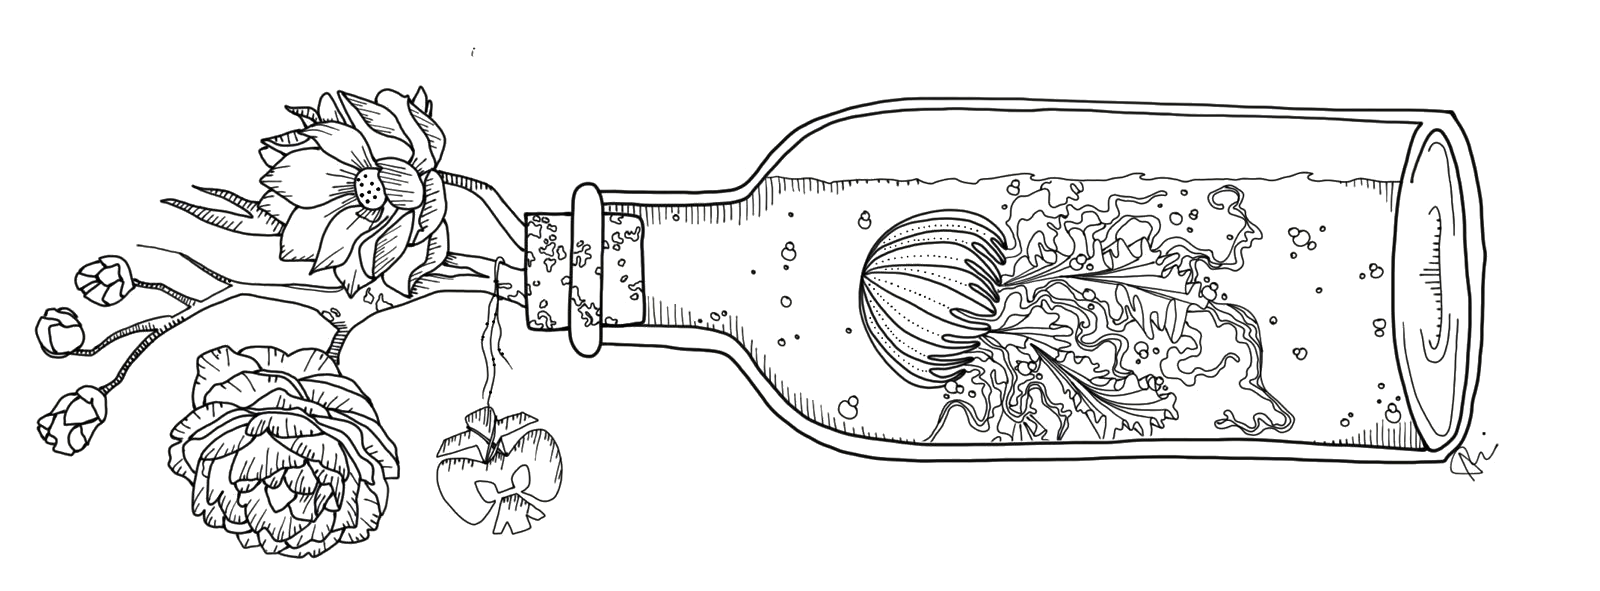
\includegraphics[scale=0.25, angle=0]{bilder/Flaschenpost.png}}}
%\end{picture}